\documentclass[25pt, a0paper, landscape, margin=0mm, innermargin=14mm,
  blockverticalspace=11mm, colspace=13mm, subcolspace=7mm]{tikzposter}

% --- Tectonic / XeTeX-safe (no fontspec, no shell-escape) ---
\usepackage[T1]{fontenc}
\usepackage{lmodern}
\usepackage{amsmath,amssymb}
\usepackage{booktabs}
\usepackage{array}
\usepackage{ragged2e}

\definecolor{ink}{RGB}{21,24,29}
\definecolor{paper}{RGB}{247,248,250}
\definecolor{ground}{RGB}{236,237,240}
\definecolor{accent}{RGB}{11,110,117}
\definecolor{violet}{RGB}{75,59,135}
\definecolor{good}{RGB}{46,115,80}
\definecolor{bad}{RGB}{156,51,46}
\definecolor{warn}{RGB}{143,98,16}

\definecolorstyle{biopunk}{}{
  \colorlet{backgroundcolor}{ground}
  \colorlet{framecolor}{ink}
  \colorlet{titlefgcolor}{ink}
  \colorlet{titlebgcolor}{ground}
  \colorlet{blocktitlebgcolor}{accent}
  \colorlet{blocktitlefgcolor}{paper}
  \colorlet{blockbodybgcolor}{white}
  \colorlet{blockbodyfgcolor}{ink}
  \colorlet{innerblocktitlebgcolor}{violet}
  \colorlet{innerblocktitlefgcolor}{paper}
  \colorlet{innerblockbodybgcolor}{paper}
  \colorlet{innerblockbodyfgcolor}{ink}
  \colorlet{notefgcolor}{ink}
  \colorlet{notebgcolor}{paper}
  \colorlet{noteframecolor}{accent}
}
\usecolorstyle{biopunk}
\usetheme{Default}
\tikzposterlatexaffectionproofoff

\newcommand{\gd}[1]{\textcolor{good}{\textbf{#1}}}
\newcommand{\bd}[1]{\textcolor{bad}{#1}}
\newcommand{\wn}[1]{\textcolor{warn}{#1}}
\newcommand{\ac}[1]{\textcolor{accent}{\textbf{#1}}}
\newcommand{\vt}[1]{\textcolor{violet}{\textbf{#1}}}

\title{\parbox{0.96\linewidth}{\centering Open-Source Continuous-Culture Bioreactors:\\[6pt]
\normalsize\mdseries A Correction, a Comparison, a Two-Instrument Proposal, and a Path to
AI-Directed Evolution}}
\author{Morgan Hough \enspace\textbullet\enspace prepared with AI assistance (Claude, Anthropic)}
\institute{\texttt{github.com/m9h/biopunk-bioreactor} \enspace\textbullet\enspace CC BY 4.0
\enspace\textbullet\enspace a reader's audit, not peer review}

\begin{document}
\maketitle

\begin{columns}

% ==================== COLUMN 1 ====================
\column{0.34}

\block{The thesis: three purposes, one lifecycle}{
Low-cost open bioreactors are compared as if they compete for one role. They do not --- the
field serves \textbf{three purposes}, stages of a lifecycle, not a ranking:
\vspace{4pt}
\begin{itemize}
  \item[\ac{proto}] \textbf{characterise} --- hold a defined state, measure richly in situ.
    \emph{Champion: Chi.Bio (an instrument).}
  \item[\vt{devo}] \textbf{evolve} --- weeks of unattended selection producing \emph{archived,
    replicated} evidence. \emph{Champion: none yet.}
  \item[\wn{bior}] \textbf{scale out} --- many reliable reactors, turnkey.
    \emph{Champions: Pioreactor, eVOLVER.}
\end{itemize}
\vspace{3pt}
\ac{proto} $\rightarrow$ \vt{devo} $\rightarrow$ \wn{bior}: prototype, evolve, produce.
A machine optimised for one is measurably worse at another --- so build purpose-built
instruments and \textbf{share the parts}, don't merge.
}

\block{Three lineages, seventy years}{
Each purpose is its own research tradition --- a founding paper and a landmark demonstration:
\par\vspace{4pt}
{\centering\small
\begin{tabular}{@{}>{\RaggedRight}p{0.09\linewidth} >{\RaggedRight}p{0.45\linewidth} >{\RaggedRight}p{0.32\linewidth}@{}}
\toprule
\textbf{} & \textbf{Founding lineage} & \textbf{Landmark} \\
\midrule
\ac{proto} & chemostat as instrument $+$ closed-loop control (Monod; Novick--Szilard 1950;
  Milias-Argeitis 2011) & optogenetic feedback holding expression $+$ growth (2016) \\[4pt]
\vt{devo} & chemostat selection $\to$ LTEE $\to$ PACE (Novick--Szilard 1950; Lenski 1991;
  Esvelt 2011) & aerobic citrate use in the LTEE (2012) \\[4pt]
\wn{bior} & continuous culture for production $\to$ arrays $\to$ eVOLVER (Herbert 1956;
  Miller 2013; Wong 2018) & eVOLVER ePACE: compact Cas9 (2022) \\
\bottomrule
\end{tabular}\par}
\vspace{5pt}
Now one \$300 device can, in principle, serve all three --- and the argument here is that it
should not try to at once.
}

\block{The instrumented reactor (\textcolor{accent}{proto})}{
\centering
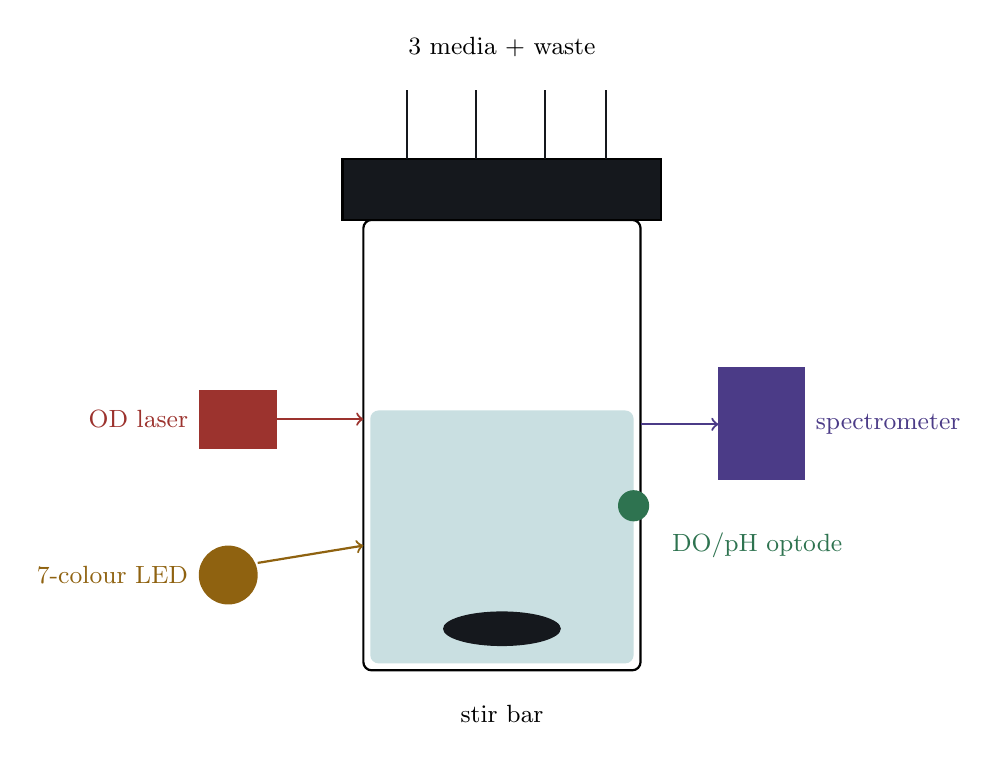
\begin{tikzpicture}[scale=2.2, line width=1.1pt, font=\small]
  % vessel + culture
  \draw[thick, fill=white, rounded corners=3pt] (0,0) rectangle (1.6,2.6);
  \fill[accent!22, rounded corners=3pt] (0.04,0.04) rectangle (1.56,1.5);
  % cap + tubes
  \draw[thick, fill=ink] (-0.12,2.6) rectangle (1.72,2.95);
  \foreach \x in {0.25,0.65,1.05,1.4} \draw[thick,ink] (\x,2.95)--(\x,3.35);
  \node[align=center] at (0.8,3.6) {3 media $+$ waste};
  % OD laser (left)
  \fill[bad] (-0.95,1.28) rectangle (-0.5,1.62);
  \draw[->,bad,thick] (-0.5,1.45)--(0,1.45);
  \node[left,text=bad] at (-0.95,1.45) {OD laser};
  % spectrometer (right)
  \fill[violet] (2.05,1.1) rectangle (2.55,1.75);
  \draw[->,violet,thick] (1.6,1.42)--(2.05,1.42);
  \node[right,text=violet] at (2.55,1.42) {spectrometer};
  % 7-colour LED (lower left)
  \fill[warn] (-0.78,0.55) circle (0.17);
  \draw[->,warn,thick] (-0.61,0.62)--(0,0.72);
  \node[left,text=warn] at (-0.95,0.55) {7-colour LED};
  % optode spot
  \fill[good] (1.56,0.95) circle (0.09);
  \node[right,text=good] at (1.72,0.72) {DO/pH optode};
  % stir bar
  \fill[ink] (0.8,0.24) ellipse (0.34 and 0.1);
  \node at (0.8,-0.25) {stir bar};
\end{tikzpicture}
\par\vspace{6pt}\raggedright\small
Non-contact optics read \emph{through the wall} --- so tubes hot-swap and stay sterile.
\ac{Eight run in parallel} on one computer.
}

% ==================== COLUMN 2 ====================
\column{0.34}

\block{Six platforms, like for like}{
{\centering\small
\begin{tabular}{@{}l ccccc@{}}
\toprule
 & \textbf{Chi.Bio} & \textbf{OpenEvo} & \textbf{Pioreactor} & \textbf{eVOLVER} & \textbf{EVE} \\
\midrule
Purpose      & \ac{proto} & \vt{devo} & \wn{bior} & \wn{bior} & \vt{devo} \\
Paper        & \gd{yes} & \gd{yes} & \bd{none} & \gd{yes} & \gd{yes} \\
Parallelism  & \gd{8} & \bd{1} & \gd{cluster} & \gd{16} & 3$+$ \\
Rich sensing & \gd{spectro.} & \bd{OD} & plugin & config. & \bd{OD} \\
Archiving    & \bd{no} & \bd{no} & \bd{no} & \bd{no} & \bd{no} \\
Cost / unit  & \$300 & \$300 & \$329 & \wn{$<$\$2k/16} & \gd{\$115} \\
Build        & \wn{PCB} & \gd{guided} & \gd{buy} & \bd{shop} & mod. \\
\bottomrule
\end{tabular}\par}
\vspace{5pt}
Two patterns: \bd{nobody archives} (the field's blind spot), and the only paperless platform is
the only pure product.
}

\block{OpenEvo: a fair correction}{
The recent OpenEvo preprint is a real contribution --- cheapest buildable selection cycler, best
manual --- but has correctable flaws:
\begin{itemize}
  \item \bd{Error:} abstract ``55\% faster'' vs.\ results ``36\% increase'' --- same data, one
    mislabelled ($7.6\!\to\!4.9$\,h is $+55\%$ rate).
  \item \bd{Error:} claims Pioreactor hardware is closed --- it is \gd{CC BY-SA 4.0} open.
  \item \bd{Method:} $n=1$, no replicates $\Rightarrow$ no causal attribution; no archiving;
    default mapper, not \texttt{breseq}, for IS-mediated deletions.
\end{itemize}
}

\block{Why \texttt{devo} has no champion}{
\vt{devo} is defined by \textbf{evidence}, not actuation. OpenEvo actuates but produces no
learnable signal. \textbf{The apparatus is the champion; a smarter vessel is not.} What the
actuator must connect to (only one is new hardware):
\vspace{2pt}
\begin{itemize}
  \item replicate manifold (borrow Pioreactor's cluster) $\to$ convergence
  \item \ac{automated chilled archiver} --- the field's missing freezer $\to$ fitness
  \item sequencing $+$ \texttt{breseq} $\to$ correct variant calls
  \item fitness loop (reuses OD hardware); selection design (growth-coupling)
\end{itemize}
}

\block{The fleet: eight chambers, one interface (\textcolor{violet}{devo} / \textcolor{warn}{bior})}{
\centering
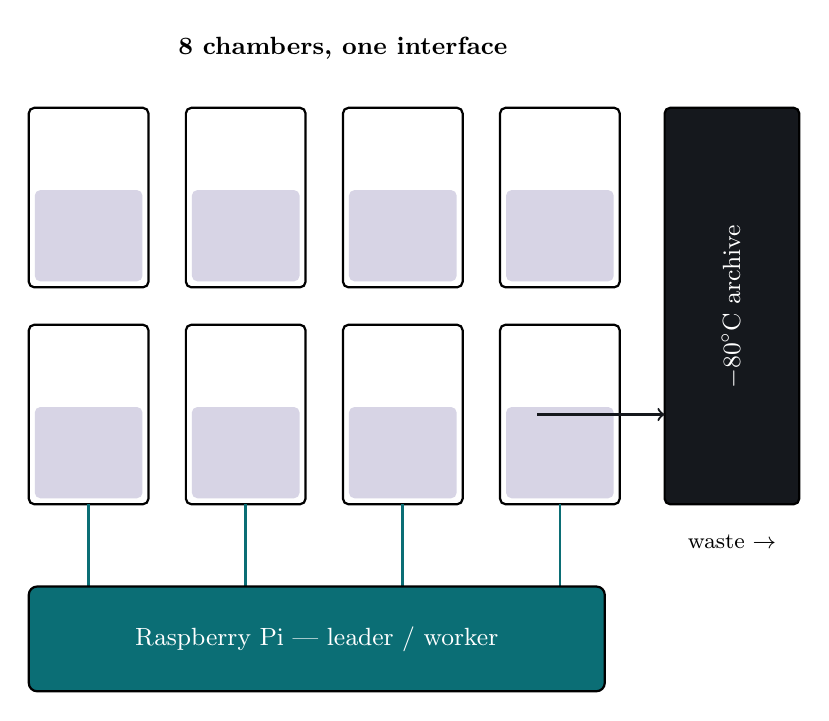
\begin{tikzpicture}[scale=1.9, line width=1pt, font=\small]
  \node at (2.1,3.15) {\textbf{8 chambers, one interface}};
  % 8 vessels, 2 rows of 4
  \foreach \i in {0,1,2,3}{
    % top row
    \draw[thick, fill=white, rounded corners=2pt] (\i*1.05,1.55) rectangle (\i*1.05+0.8,2.75);
    \fill[violet!22, rounded corners=2pt] (\i*1.05+0.04,1.59) rectangle (\i*1.05+0.76,2.2);
    % bottom row
    \draw[thick, fill=white, rounded corners=2pt] (\i*1.05,0.1) rectangle (\i*1.05+0.8,1.3);
    \fill[violet!22, rounded corners=2pt] (\i*1.05+0.04,0.14) rectangle (\i*1.05+0.76,0.75);
    % feeders from controller
    \draw[accent] (\i*1.05+0.4,-0.45)--(\i*1.05+0.4,0.1);
  }
  % controller
  \draw[thick, fill=accent, rounded corners=3pt] (0,-1.15) rectangle (3.85,-0.45);
  \node[white] at (1.925,-0.8) {Raspberry Pi --- leader / worker};
  % archiver
  \draw[thick, fill=ink, rounded corners=2pt] (4.25,0.1) rectangle (5.15,2.75);
  \node[white, rotate=90, font=\small] at (4.7,1.42) {$-80^{\circ}$C archive};
  \draw[->,ink,thick] (3.4,0.7)--(4.25,0.7);
  \node[align=center, font=\footnotesize] at (4.7,-0.15) {waste $\to$};
\end{tikzpicture}
\par\vspace{6pt}\raggedright\small
Many cheap chambers under one controller, with the \ac{automated chilled archiver} on the waste
line --- the field's missing freezer, and what makes fitness measurable.
}

% ==================== COLUMN 3 ====================
\column{0.32}

\block{Three biopunk builds \& what they buy}{
\textbf{\ac{proto --- updated Chi.Bio.}} Chi.Bio core $+$ OpenEvo gas vessel $+$ through-wall
DO/pH optodes $+$ C12880MA spectrometer $+$ Pi. \emph{Benefit:} the most complete non-contact
in-situ characterisation instrument in open hardware.
\par\vspace{6pt}
\textbf{\vt{devo --- evolution $+$ evidence.}} Pioreactor cluster (or OpenEvo base) $+$ 3-media
fluidics $+$ replicate fleet $+$ \ac{archiver} $+$ \texttt{breseq} $+$ fitness assay.
\emph{Benefit:} fills the empty \vt{devo} slot --- first open platform with \emph{publishable}
evolution evidence.
\par\vspace{6pt}
\textbf{\wn{bior --- Pioreactor $+$ add-ons.}} Buy the cluster; add the shared optode module
(plugin), eVOLVER sleeves only where needed. \emph{Benefit:} reliable parallel cultivation
now --- mostly bought, not built.
\par\vspace{6pt}
Three configurations of \textbf{one shared platform}: Raspberry Pi $+$ one module footprint $+$
one calibration reference.
}

\block{The goal: AI-directed evolution}{
OpenEvo \emph{pitched} ``AI to supervise the evolution'' but built only the actuator.
\textbf{The observation layer an AI needs \emph{is} the evidence apparatus} --- so
\ac{apparatus $=$ champion, AI $=$ autopilot}; build the apparatus first, then close the loop:
\vspace{2pt}
\begin{itemize}
  \item \textbf{observe} growth $+$ fitness $+$ genotype (\texttt{breseq})
  \item \textbf{act} on media / light / dilution $+$ \vt{CRISPR-targeted mutation} (EvolvR, an
    \textbf{IGI} tool)
  \item \textbf{learn} rule-based $\to$ Bayesian opt $\to$ RL, across the fleet
\end{itemize}
CRISPR sharpens every layer: EvolvR (targeted diversification), CAMERA (in-cell recorder),
Cas-coupled selection. \emph{Prove it: AI-directed vs.\ fixed schedule, same target.}
}

\block{Take-aways}{
\begin{enumerate}
  \item Three purposes, not one contest --- different winners.
  \item Evolution has \bd{no champion}: nobody archives or replicates. \emph{That is the opening.}
  \item The killer feature nobody has shipped: an \ac{automated chilled archiver}.
  \item Build the apparatus first; the AI autopilot follows.
\end{enumerate}
\vspace{3pt}
\centering \Large\ac{github.com/m9h/biopunk-bioreactor}\\[3pt]
\normalsize public $\cdot$ CC BY 4.0 $\cdot$ corrections with citations welcome
}

\end{columns}
\end{document}
